\documentclass[handout]{beamer}\usepackage[]{graphicx}\usepackage[]{color}
%% maxwidth is the original width if it is less than linewidth
%% otherwise use linewidth (to make sure the graphics do not exceed the margin)
\makeatletter
\def\maxwidth{ %
  \ifdim\Gin@nat@width>\linewidth
    \linewidth
  \else
    \Gin@nat@width
  \fi
}
\makeatother

\definecolor{fgcolor}{rgb}{0.345, 0.345, 0.345}
\newcommand{\hlnum}[1]{\textcolor[rgb]{0.686,0.059,0.569}{#1}}%
\newcommand{\hlstr}[1]{\textcolor[rgb]{0.192,0.494,0.8}{#1}}%
\newcommand{\hlcom}[1]{\textcolor[rgb]{0.678,0.584,0.686}{\textit{#1}}}%
\newcommand{\hlopt}[1]{\textcolor[rgb]{0,0,0}{#1}}%
\newcommand{\hlstd}[1]{\textcolor[rgb]{0.345,0.345,0.345}{#1}}%
\newcommand{\hlkwa}[1]{\textcolor[rgb]{0.161,0.373,0.58}{\textbf{#1}}}%
\newcommand{\hlkwb}[1]{\textcolor[rgb]{0.69,0.353,0.396}{#1}}%
\newcommand{\hlkwc}[1]{\textcolor[rgb]{0.333,0.667,0.333}{#1}}%
\newcommand{\hlkwd}[1]{\textcolor[rgb]{0.737,0.353,0.396}{\textbf{#1}}}%
\let\hlipl\hlkwb

\usepackage{framed}
\makeatletter
\newenvironment{kframe}{%
 \def\at@end@of@kframe{}%
 \ifinner\ifhmode%
  \def\at@end@of@kframe{\end{minipage}}%
  \begin{minipage}{\columnwidth}%
 \fi\fi%
 \def\FrameCommand##1{\hskip\@totalleftmargin \hskip-\fboxsep
 \colorbox{shadecolor}{##1}\hskip-\fboxsep
     % There is no \\@totalrightmargin, so:
     \hskip-\linewidth \hskip-\@totalleftmargin \hskip\columnwidth}%
 \MakeFramed {\advance\hsize-\width
   \@totalleftmargin\z@ \linewidth\hsize
   \@setminipage}}%
 {\par\unskip\endMakeFramed%
 \at@end@of@kframe}
\makeatother

\definecolor{shadecolor}{rgb}{.97, .97, .97}
\definecolor{messagecolor}{rgb}{0, 0, 0}
\definecolor{warningcolor}{rgb}{1, 0, 1}
\definecolor{errorcolor}{rgb}{1, 0, 0}
\newenvironment{knitrout}{}{} % an empty environment to be redefined in TeX

\usepackage{alltt}

\usepackage{default}
\usepackage{animate} %need the animate.sty file 
\usepackage{graphicx}
%\graphicspath{{/home/sahir/Dropbox/jobs/laval/minicours/slides/}}
\usepackage{hyperref, url}
%\usepackage[round,sort]{natbib}   % bibliography omit 'round' option if you prefer square brackets
%\bibliographystyle{apalike}
\usepackage{biblatex}
\bibliography{bib.bib}
% Removes icon in bibliography
\setbeamertemplate{bibliography item}[text]

\usepackage[normalem]{ulem}

\setbeamertemplate{theorems}[numbered]
\usepackage[final]{pdfpages}



%\newtheorem{prop}{Proposition}
%\newenvironment{theoremc}[1]
%{\begin{shaded}\begin{theorem}[#1]}
%		{\end{theorem}\end{shaded}}

%\newtheorem{examplefirst}{Example}
%\newtheorem{examplesecond}{Example}
%\newenvironment<>{examplefirst}[1][]{%
%	\setbeamercolor{block title example}{bg=lightgray}%
%	\begin{example}#2[#1]}{\end{example}}
%\newenvironment<>{examplesecond}[1][]{%
%	\setbeamercolor{block title example}{fg=white,bg=blue!75!black}%
%	\begin{example}#2[#1]}{\end{example}}	

%\usepackage{amsthm}


\usepackage[figurename=Fig.]{caption}
\usepackage{subfig}
\usepackage{tikz, pgfplots,epsfig}
\usetikzlibrary{arrows,shapes.geometric}
\usepackage{color, colortbl,xcolor}
\definecolor{lightgray}{RGB}{200,200,200}
\definecolor{palegray}{RGB}{221,221,221}
\definecolor{myblue}{RGB}{0,89,179}
\usepackage{comment}
\setbeamercolor{frametitle}{fg=myblue}
\setbeamercolor{section in head/foot}{bg=myblue, fg=white}
\setbeamercolor{author in head/foot}{bg=myblue}
\setbeamercolor{date in head/foot}{bg=myblue}

\usepackage{shadethm}
%\colorlet{shadecolor}{blue!15}
\colorlet{shadecolor}{palegray}
%\setlength{\shadeboxrule}{.4pt}

\newshadetheorem{thm}{Theorem}
\newshadetheorem{defm}{Definition}
\newshadetheorem{exm}{Exercise}
\newshadetheorem{remarkm}{Remark}
%\definecolor{shadethmcolor}{HTML}{EDF8FF}
\definecolor{shadethmcolor}{RGB}{221,221,221}
%\definecolor{shaderulecolor}{HTML}{45CFFF}
\definecolor{shaderulecolor}{RGB}{0,89,179}
\setlength{\shadeboxrule}{.4pt}


\usepackage{array}
\newcolumntype{L}{>{\centering\arraybackslash}m{3cm}} % used for text wrapping in ctable
\usepackage{ctable}
\usepackage[utf8]{inputenc}
\usepackage{fontenc}
\usepackage{pifont}% http://ctan.org/pkg/pifont
\newcommand{\cmark}{\ding{51}}%
\newcommand{\xmark}{\ding{55}}%
\def\widebar#1{\overline{#1}}
\definecolor{whitesmoke}{rgb}{0.96, 0.96, 0.96}

\usepackage{amssymb}
\usepackage{amsmath}

\usepackage{bm}
\def\transpose{{\sf{T}}}
\def\E{{\skew0\bm{E}}}
\def\Xvec{{\skew0\bm{X}}}
\def\Xveca{{\skew0\bm{X}}_1}
\def\Xvecb{{\skew0\bm{X}}_2}

\def\Yvec{{\skew0\bm{Y}}}
\def\bmY{{\skew0\bm{Y}}}
\def\bmX{{\skew0\bm{X}}}
\def\bmy{{\skew0\bm{y}}}
\def\bmG{{\skew0\bm{G}}}
\def\bmS{{\skew0\bm{S}}}
\def\bmA{{\skew0\bm{A}}}
\def\bmB{{\skew0\bm{B}}}
\def\bmD{{\skew0\bm{D}}}
\def\bmI{{\skew0\bm{I}}}
\def\bmV{{\skew0\bm{V}}}
\def\bmU{{\skew0\bm{U}}}
\def\bv{{\skew0\bm{v}}}
\def\bw{{\skew0\bm{w}}}
\def\bmm{{\skew0\bm{m}}}
\def\bmzero{{\skew0\bm{0}}}
\def\bx{{\skew0\bm{x}}}
\def\xveca{{\skew0\bm{x}}_1}
\def\xvecb{{\skew0\bm{x}}_2}

\def\N{{\skew0\mathcal{N}}}
\def\T{{\small T}}

\def\mvec{{\skew0\bm{m}}}
\def\bmmu{{\skew0\bm{\mu}}}
\def\muvec{{\skew0\bm{\mu}}}
\def\balpha{{\skew0\bm{\alpha}}}
\def\bbeta{{\skew0\bm{\beta}}}
\def\bmtheta{{\skew0\bm{\theta}}}
\def\btheta{{\skew0\bm{\theta}}}

\def\cvec{{\skew0\mathbf{c}}}

\def\Xbar{\overline{X}}

\definecolor{lightgray}{rgb}{0.91,0.91,0.91}
\definecolor{purpleblue}{rgb}{0.50,0.50,1.00}



\usepackage{fontspec}
%\setsansfont{Fira Sans}
%\setmonofont{Fira Mono}
\setsansfont[ItalicFont={Fira Sans Light Italic},BoldFont={Fira Sans},BoldItalicFont={Fira Sans Italic}]{Fira Sans Light}
\setmonofont[BoldFont={Fira Mono Medium}]{Fira Mono}


\setbeamercolor{itemize item}{fg=myblue}
\setbeamertemplate{itemize item}[square]

\setbeamertemplate{navigation symbols}{\usebeamercolor[fg]{title in head/foot}\usebeamerfont{title in head/foot}\insertframenumber}
\setbeamertemplate{footline}{}

\newtheorem{proposition}[theorem]{Proposition}
\newtheorem{exercise}[theorem]{Exercise}

\titlegraphic{\hfill
\includegraphics[height=1cm]{mcgill_logo.png}}


%% You also use hyperref, and pick colors 
\hypersetup{colorlinks,citecolor=orange,filecolor=red,linkcolor=brown,urlcolor=blue}

\newcommand {\framedgraphiccaption}[2] {
	\begin{figure}
		\centering
		\includegraphics[width=\textwidth,height=0.8\textheight,keepaspectratio]{#1}
		\caption{#2}
	\end{figure}
}

\newcommand {\framedgraphic}[1] {
	\begin{figure}
		\centering
		\includegraphics[width=\textwidth,height=0.9\textheight,keepaspectratio]{#1}
	\end{figure}
}


\AtBeginSection[]{
	\begin{frame}
	\vfill
	\centering
	\begin{beamercolorbox}[sep=8pt,center,shadow=true,rounded=true]{title}
		\usebeamerfont{title}\insertsectionhead\par%
	\end{beamercolorbox}
	\vfill
\end{frame}
}

\newcommand\Wider[2][3em]{%
\makebox[\linewidth][c]{%
	\begin{minipage}{\dimexpr\textwidth+#1\relax}
		\raggedright#2
	\end{minipage}%
}%
}



\newcommand{\blue}[1]{\textcolor{blue}{#1}}
\newcommand{\red}[1]{\textcolor{red}{#1}}
%\makeatother

\usepackage{xparse}
\NewDocumentCommand\mylist{>{\SplitList{;}}m}
{
\begin{itemize}
	\ProcessList{#1}{ \insertitem }
\end{itemize}
}
\NewDocumentCommand\mynum{>{\SplitList{;}}m}
{
\begin{enumerate}
	\ProcessList{#1}{ \insertitem }
\end{enumerate}
}
\newcommand\insertitem[1]{\item #1}

\newcommand\FrameText[1]{%
\begin{textblock*}{\paperwidth}(0pt,\textheight)
	\raggedright #1\hspace{.5em}
\end{textblock*}}
\IfFileExists{upquote.sty}{\usepackage{upquote}}{}
\begin{document}
%\sffamily



%\title{Introduction to Regression Trees}
%\author{Sahir Bhatnagar \inst{1}}
%\author[shortname]{Sahir Rai Bhatnagar, PhD Candidate (Biostatistics) }
%\institute[shortinst]{Department of Epidemiology, Biostatistics and Occupational Health}

\title{Inference about a Population Rate ($\lambda$)}
\subtitle{\href{https://www.dropbox.com/s/b5q7vqo2ev6k2me/EPIB607intensity-model-inference-plan-2018.pdf?dl=0}{JH notes on rates}}
\author{Sahir Bhatnagar and James Hanley}
\institute{
	EPIB 607\\
	Department of Epidemiology, Biostatistics, and Occupational Health\\
	McGill University\\
	
	\vspace{0.1 in}
	
	\texttt{sahir.bhatnagar@mcgill.ca}\\
	\texttt{\url{https://sahirbhatnagar.com/EPIB607/}}}

%\date

\maketitle

\section{Poisson Model for Sampling Variability of a Count in a Given Amount of ``Experience''}

\begin{frame}{Motivating example: Demand for medical care}

\begin{itemize}
	\setlength\itemsep{1em}
	\item Data from the US National Medical	Expenditure Survey (NMES) for 1987/88
	\item 4406 individuals, aged 66 and over, who are covered by Medicare, a public insurance program
	\item The objective of the study was to model the demand for medical care - as captured by \underline{the number} of physician/non-physician office and hospital outpatient visits - by the covariates available for the patients.
\end{itemize}

\end{frame}


\begin{frame}[fragile]{Motivating example: Demand for medical care}

\vspace*{-0.2in}

\begin{knitrout}\scriptsize
\definecolor{shadecolor}{rgb}{0.969, 0.969, 0.969}\color{fgcolor}

{\centering 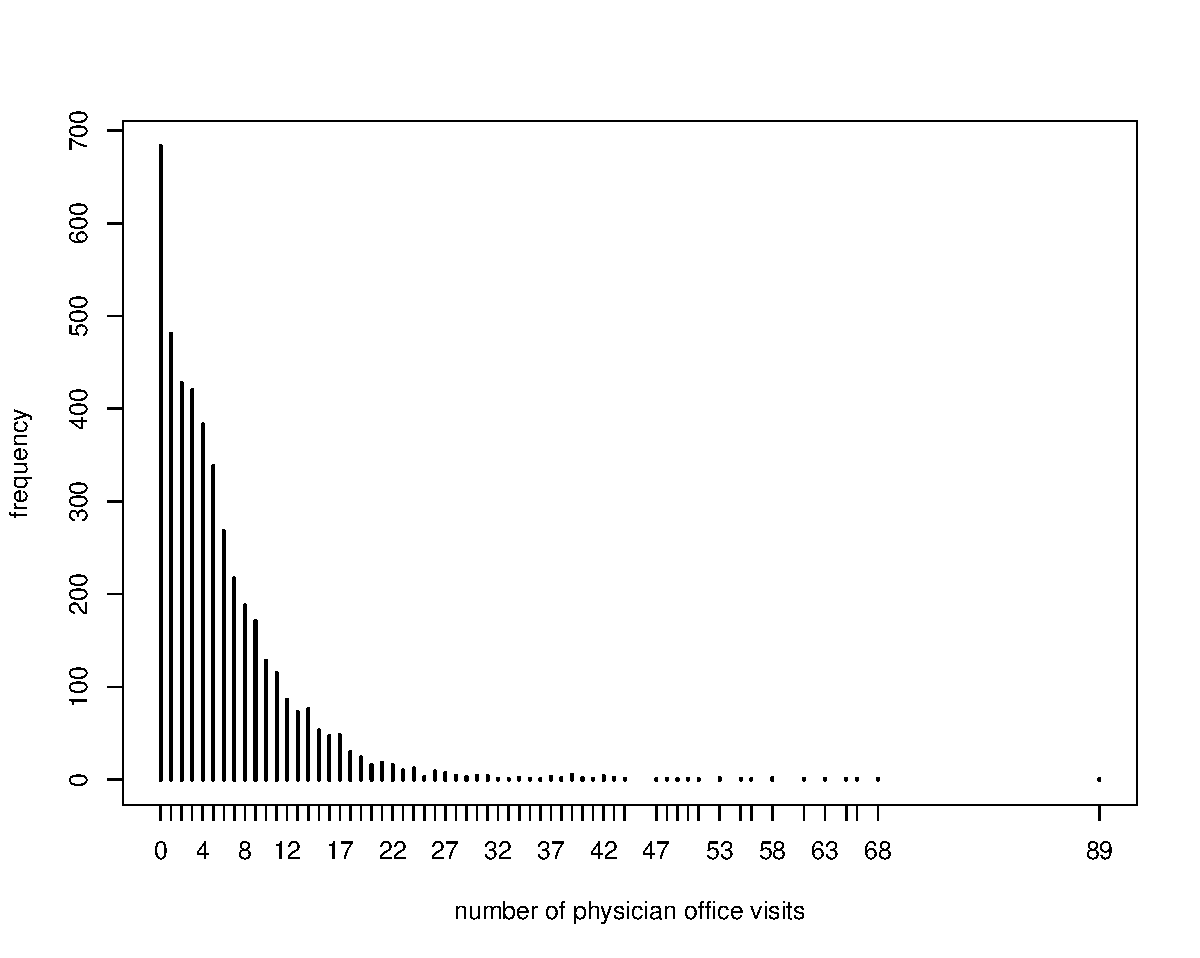
\includegraphics[width=1\linewidth]{figure/unnamed-chunk-1-1} 

}



\end{knitrout}


\end{frame}


\begin{frame}{Some observations about the previous plot}

\begin{itemize}
\setlength\itemsep{1em}
\item Discrete outcome $\to$ 1, 2, 3, ... visits \pause 
\item There are rare events, e.g. 1 individual with 89 visits \pause 
\item The data are far from normally distributed \pause
\item Can theoretically go on forever
\end{itemize}

\end{frame}

\begin{frame}{The Poisson Distribution}


\begin{itemize}
\setlength\itemsep{1em}
\item The binomial distribution was derived by starting with an experiment consisting of trials or draws and applying the laws of probability to various outcomes of the experiment. \pause 
\item There is no simple experiment on which the Poisson distribution is based, although we will shortly describe how it can be obtained by certain limiting operations.
\end{itemize}

\end{frame}

\begin{frame}
\frametitle{The Poisson Distribution: what it is, and features}

\begin{itemize}
\small
\setlength\itemsep{1em}
\item The (infinite number of) probabilities $P_{0}, P_{1}, ..., P_{y}, ..., $ of observing 
$Y = 0, 1, 2, \dots , y, \dots $ events in a given amount of ``experience.'' \pause

\item These probabilities, $P(Y = k) \to$ \texttt{dpois()}, are governed by a single parameter, the mean $E[Y] = \mu$ which represents the expected \textbf{number} of events in the amount of experience actually studied.\pause 

\item We say that a random variable $Y \sim \textrm{Poisson}(\mu)$ distribution if 

\[ P(Y=k) = \frac{\mu^k}{k!}e^{-\mu}, \quad k = 0, 1, 2, \ldots\]
\pause 

\item Note: in \texttt{dpois()} $\mu$ is referred to as \texttt{lambda}

\item Note the distinction between $\mu$ and $\lambda$
\begin{itemize}
\item $\mu$: expected \textbf{number} of events
\item $\lambda$: \textbf{rate} parameter
\end{itemize}
\end{itemize}
\end{frame}

\begin{frame}[fragile]{The probability mass function for $\mu=0.5$}

\begin{knitrout}\scriptsize
\definecolor{shadecolor}{rgb}{0.969, 0.969, 0.969}\color{fgcolor}
\begin{alltt}
\hlkwd{dpois}\hlstd{(}\hlkwc{x} \hlstd{=} \hlnum{0}\hlopt{:}\hlnum{15}\hlstd{,} \hlkwc{lambda} \hlstd{=} \hlnum{0.5}\hlstd{)}
\end{alltt}

\end{knitrout}

\vspace*{-0.5in}

\begin{knitrout}\scriptsize
\definecolor{shadecolor}{rgb}{0.969, 0.969, 0.969}\color{fgcolor}

{\centering 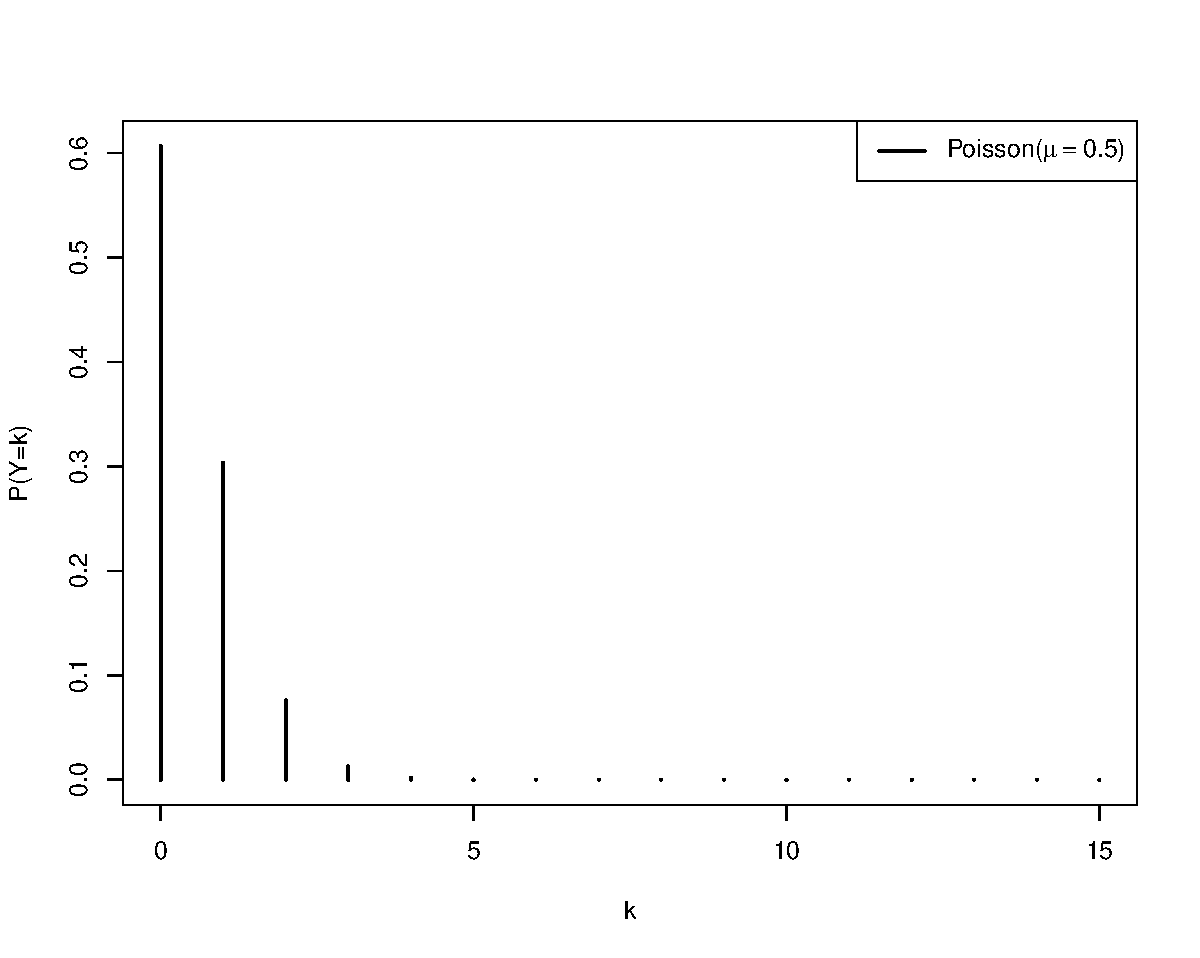
\includegraphics[width=1\linewidth]{figure/unnamed-chunk-3-1} 

}



\end{knitrout}

\end{frame}


\begin{frame}[fragile]{The probability mass function for $\mu=10$}

\begin{knitrout}\scriptsize
\definecolor{shadecolor}{rgb}{0.969, 0.969, 0.969}\color{fgcolor}
\begin{alltt}
\hlkwd{dpois}\hlstd{(}\hlkwc{x} \hlstd{=} \hlnum{0}\hlopt{:}\hlnum{15}\hlstd{,} \hlkwc{lambda} \hlstd{=} \hlnum{10}\hlstd{)}
\end{alltt}

\end{knitrout}

\vspace*{-0.5in}

\begin{knitrout}\scriptsize
\definecolor{shadecolor}{rgb}{0.969, 0.969, 0.969}\color{fgcolor}

{\centering 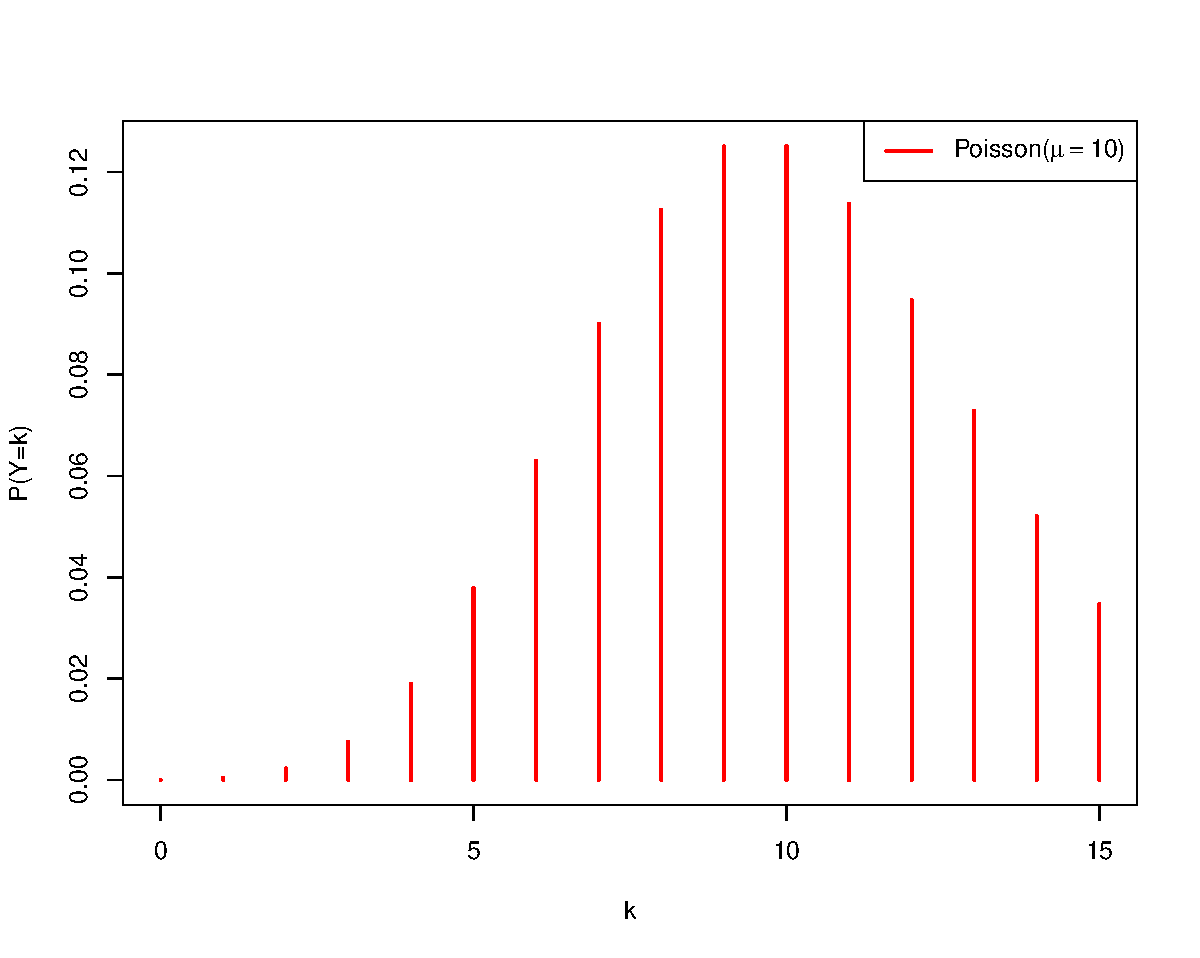
\includegraphics[width=1\linewidth]{figure/unnamed-chunk-5-1} 

}



\end{knitrout}

\end{frame}


\begin{frame}[fragile]{The probability mass function}

\begin{knitrout}\scriptsize
\definecolor{shadecolor}{rgb}{0.969, 0.969, 0.969}\color{fgcolor}

{\centering 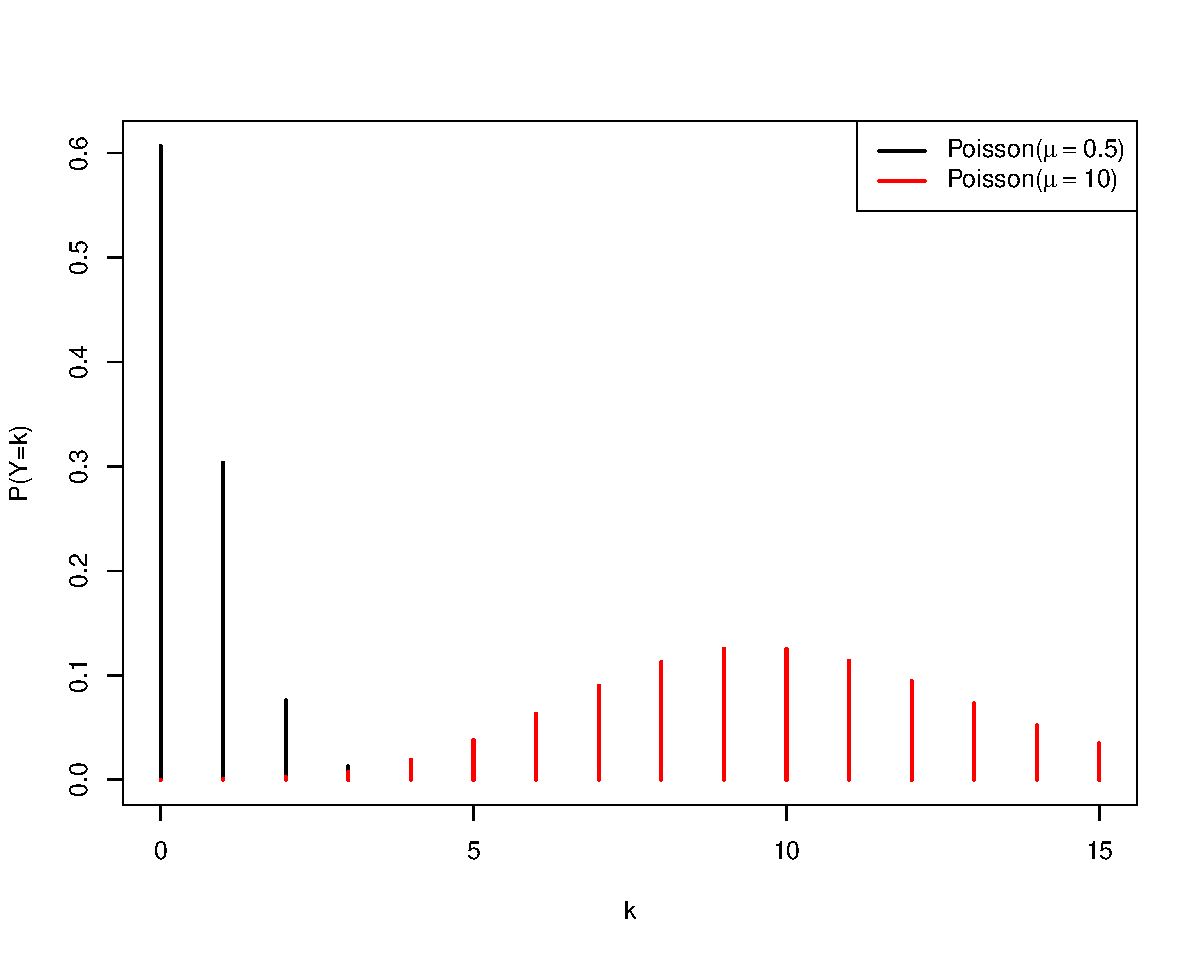
\includegraphics[width=1\linewidth]{figure/unnamed-chunk-6-1} 

}



\end{knitrout}

\end{frame}


\begin{frame}
\frametitle{The Poisson Distribution: what it is, and features}

\begin{itemize}
\setlength\itemsep{2em}
\item  $\sigma^2_Y =  \mu \ \to \ \ \sigma_Y =  \sqrt{\mu}.$ \pause
\item  Approximated by $\mathcal{N}(\mu, \sqrt{\mu})$ when $\mu >> 10$ \pause 
\item Open-ended (unlike Binomial), but in practice, has finite range. 

\item Poisson data sometimes called "numerator only":  (unlike Binomial) may not ``see'' or  count ``non-events''
\end{itemize}
\end{frame}


\begin{frame}[fragile]{Normal approximation to Poisson is the CLT in action}
\begin{knitrout}\scriptsize
\definecolor{shadecolor}{rgb}{0.969, 0.969, 0.969}\color{fgcolor}

{\centering 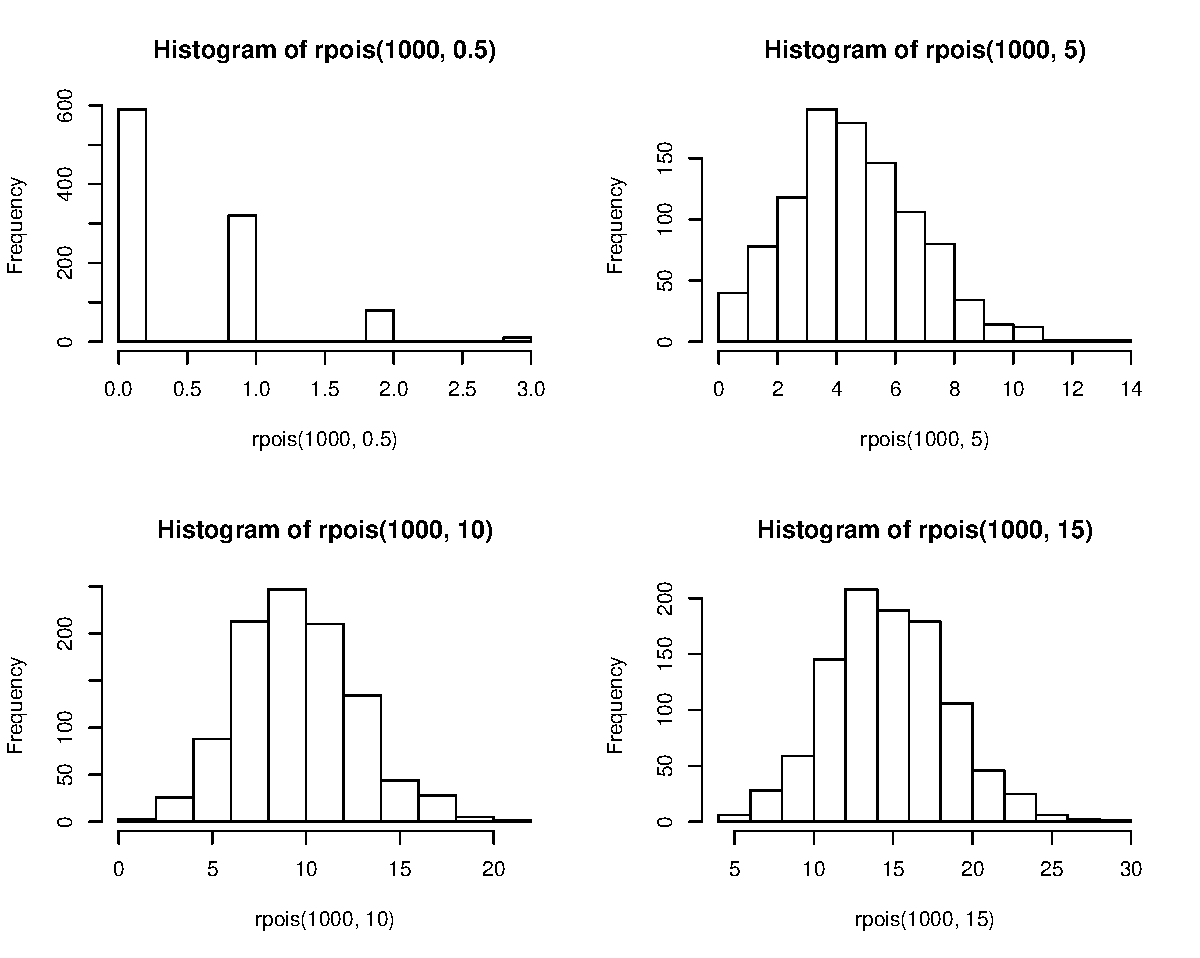
\includegraphics[width=1\linewidth]{figure/unnamed-chunk-7-1} 

}



\end{knitrout}
\end{frame}	



\begin{frame}
\frametitle{How it arises}

\begin{itemize}
\setlength\itemsep{1em}
\item  Count of events or items that \underline{occur randomly}, with \underline{low homogeneous intensity}, in time, space, or `item'-time (e.g. person--time). \pause 
\item Binomial($n,\pi$) when $n \rightarrow \infty\textrm{ and } \pi \rightarrow 0,$ but $n \times \pi = \mu$ is finite.\pause 
\item $Y\sim Poisson(\mu_Y)$ if time ($T$) between events follows an $T \sim \textrm{Exponential}(\mu_{T} = 1/\mu_{Y}).$ 
{ \scriptsize   \url{http://www.epi.mcgill.ca/hanley/bios601/Intensity-Rate/Randomness_poisson.pdf}} \pause
\item  As sum of $\ge 2$  \textit{independent} Poisson random variables, 
with same \textbf{or different} $\mu$'s: \newline 
$Y_{1} \sim \textrm{Poisson}(\mu_{1}) \: \:   
Y_{2} \sim \textrm{Poisson}(\mu_{2}) \Rightarrow Y = Y_{1} + Y_{2} \sim \textrm{Poisson}(\mu_{1}+\mu_{2}).$
\end{itemize}
\end{frame}


\begin{frame}{Poisson distribution as a limit}

The rationale for using the Poisson distribution in many situations is provided by the following proposition.

\vspace*{0.5in}

\begin{proposition}[Limit of a binomial is Poisson]
Suppose that $Y \sim Binomial(n,\pi)$. If we let $\pi = \mu/n$, then as $n \rightarrow \infty$, $Binomial(n,\pi) \rightarrow Poisson(\mu)$. Another way of saying this: for large $n$ and small $\pi$, we can approximate the $Binomial(n,\pi)$ probability by the $Poisson(\mu = n\pi)$. 
\end{proposition}

\end{frame}


\begin{frame}{Poisson approximation to the Binomial}


\begin{knitrout}\scriptsize
\definecolor{shadecolor}{rgb}{0.969, 0.969, 0.969}\color{fgcolor}

{\centering 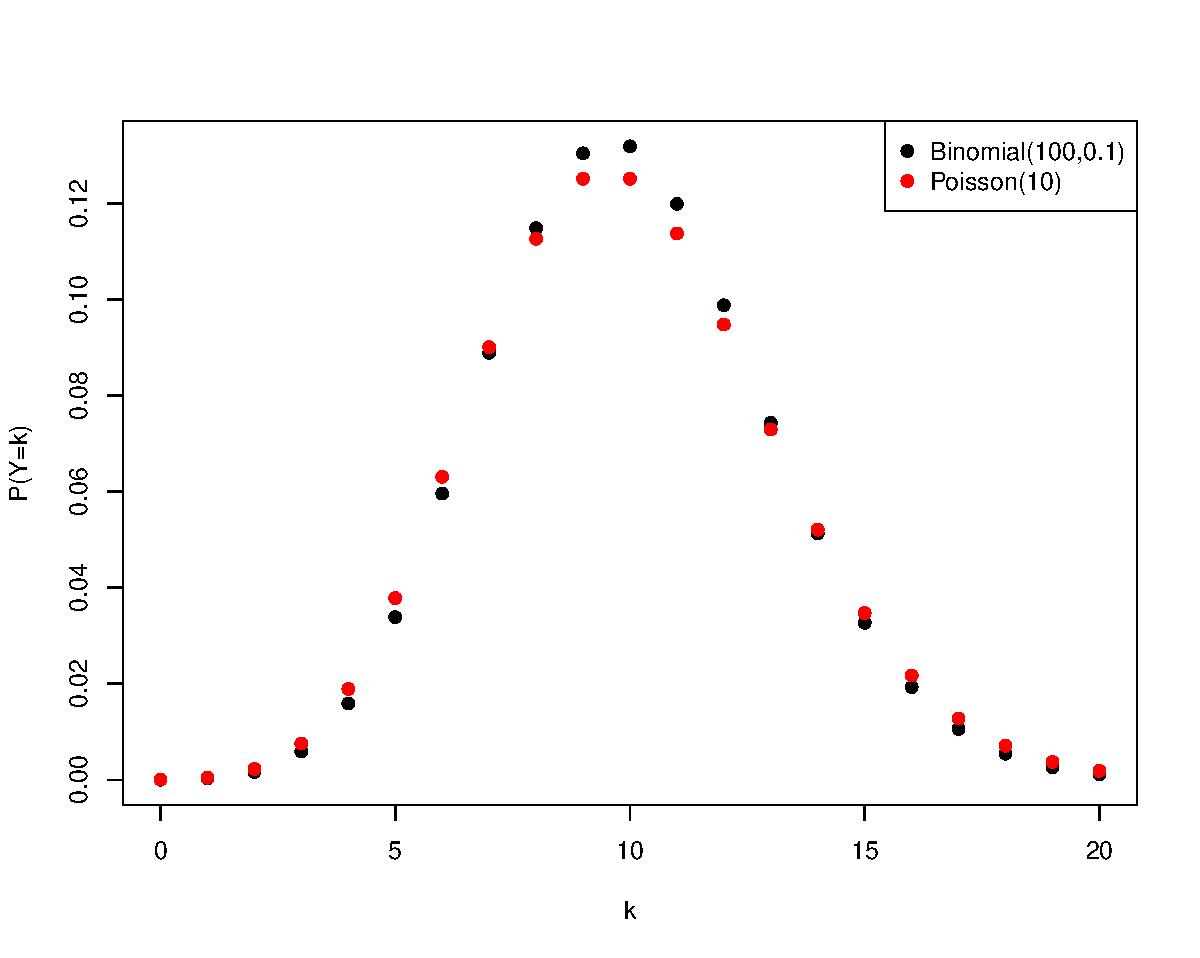
\includegraphics[width=1\linewidth]{figure/unnamed-chunk-8-1} 

}



\end{knitrout}

\end{frame}


\begin{frame}
\frametitle{Examples}

\begin{itemize}
\setlength\itemsep{0.5em}
\item numbers of asbestos fibres
\item deaths from horse kicks*
\item needle-stick or other percutaneous injuries
\item bus-driver accidents*
\item twin-pairs*
\item radioactive disintegrations*
\item flying-bomb hits*
\item white blood cells
\item typographical errors
\item cell occupants -- in a given volume, area, line-length, population-time, time, etc. 
\footnote{\footnotesize * included in \url{http://www.epi.mcgill.ca/hanley/bios601/Intensity-Rate/}}
\end{itemize}
\end{frame}



\begin{frame}
\frametitle{}
\begin{figure}[h]
\begin{center}
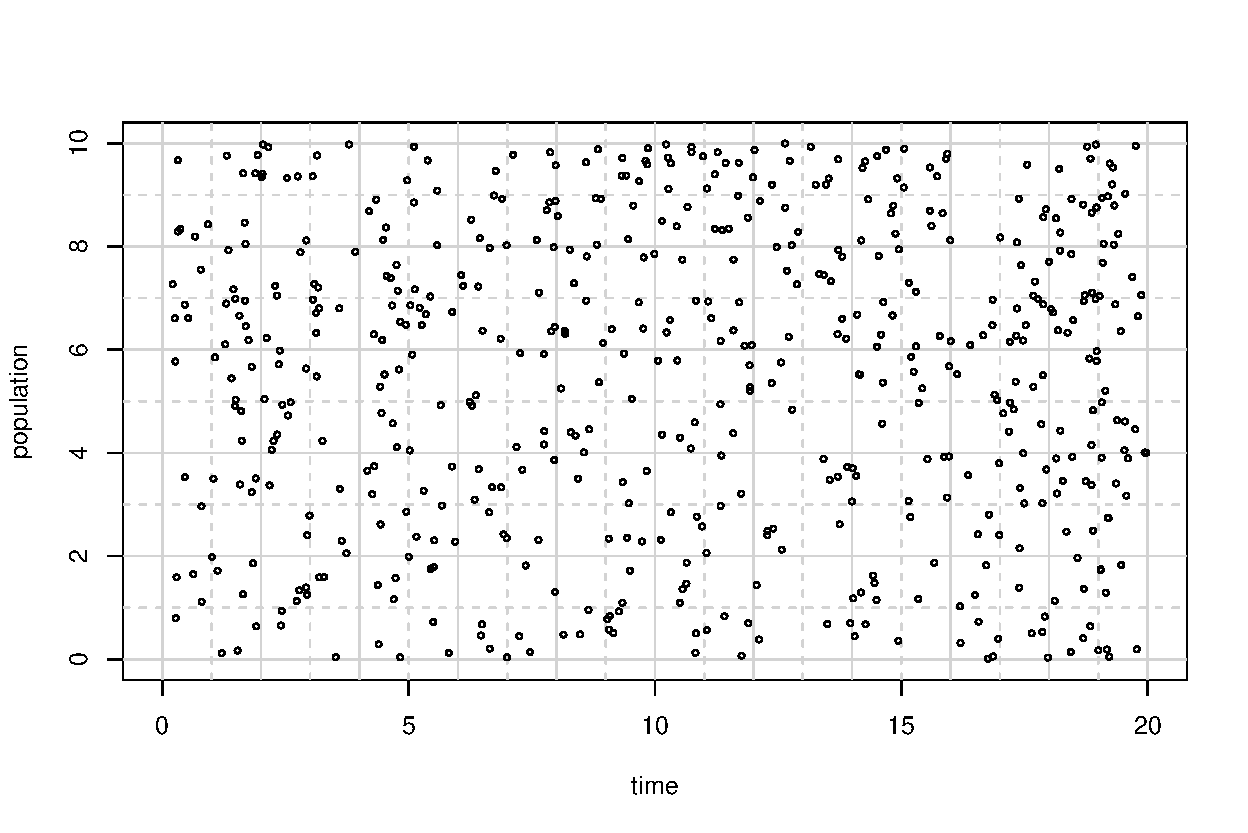
\includegraphics[width=3.9in,height=2.6in]{DotsinPopulationTime64.pdf}
\caption{Events in Population-Time randomly generated from intensities that are constant within (2 squares high by 2 squares wide) `panels', but vary between such panels. In Epidemiology, each square might represent a number of units of population-time, and each dot an event.}
\end{center}
\end{figure}
\end{frame}

\begin{frame}
\frametitle{}
\begin{figure}[h]
\begin{center}
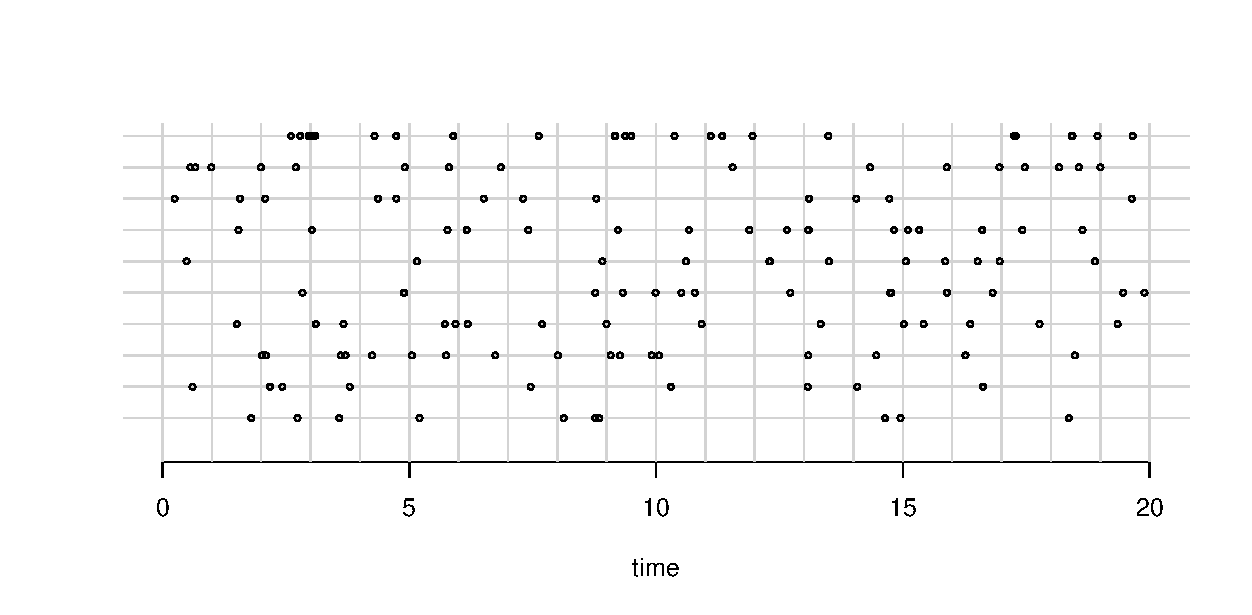
\includegraphics[width=4in,height=2in]{timeStrips63.pdf}
\caption{Events in Time: 10 examples, randomly generated from constant over time intensities. Simulated with 1000 Bernoulli$(\tiny{\textrm{small }\pi})$'s per time unit.}
\end{center}
\end{figure}
\end{frame}


\begin{frame}
\frametitle{Does the Poisson Distribution apply to.. ?}

\begin{enumerate}
\setlength\itemsep{0.9em}
\item Yearly variations in numbers of persons killed in	plane crashes 
\item Daily variations in numbers of births
\item Weekly variations in numbers of births
\item Daily variations in numbers of deaths
\item Daily variations in numbers of traffic accidents
\item Variations across cookies/pizzas in numbers of chocolate chips/olives
\end{enumerate}
\end{frame}




\section{Inference regarding $\mu$, based on observed count $y$}

\begin{frame}[fragile]{Confidence interval for $\mu$}
\begin{itemize}
\setlength\itemsep{2em}
\item If the CLT hasn't kicked in, then the usual CI might not be appropriate: $$\textrm{point-estimate} \pm z^\star  \times \textrm{standard error}$$

\begin{knitrout}\scriptsize
\definecolor{shadecolor}{rgb}{0.969, 0.969, 0.969}\color{fgcolor}
\begin{alltt}
\hlstd{mosaic}\hlopt{::}\hlkwd{xqpois}\hlstd{(}\hlkwd{c}\hlstd{(}\hlnum{0.025}\hlstd{,} \hlnum{0.975}\hlstd{),} \hlkwc{lambda} \hlstd{=} \hlnum{6}\hlstd{)}
\end{alltt}


{\centering 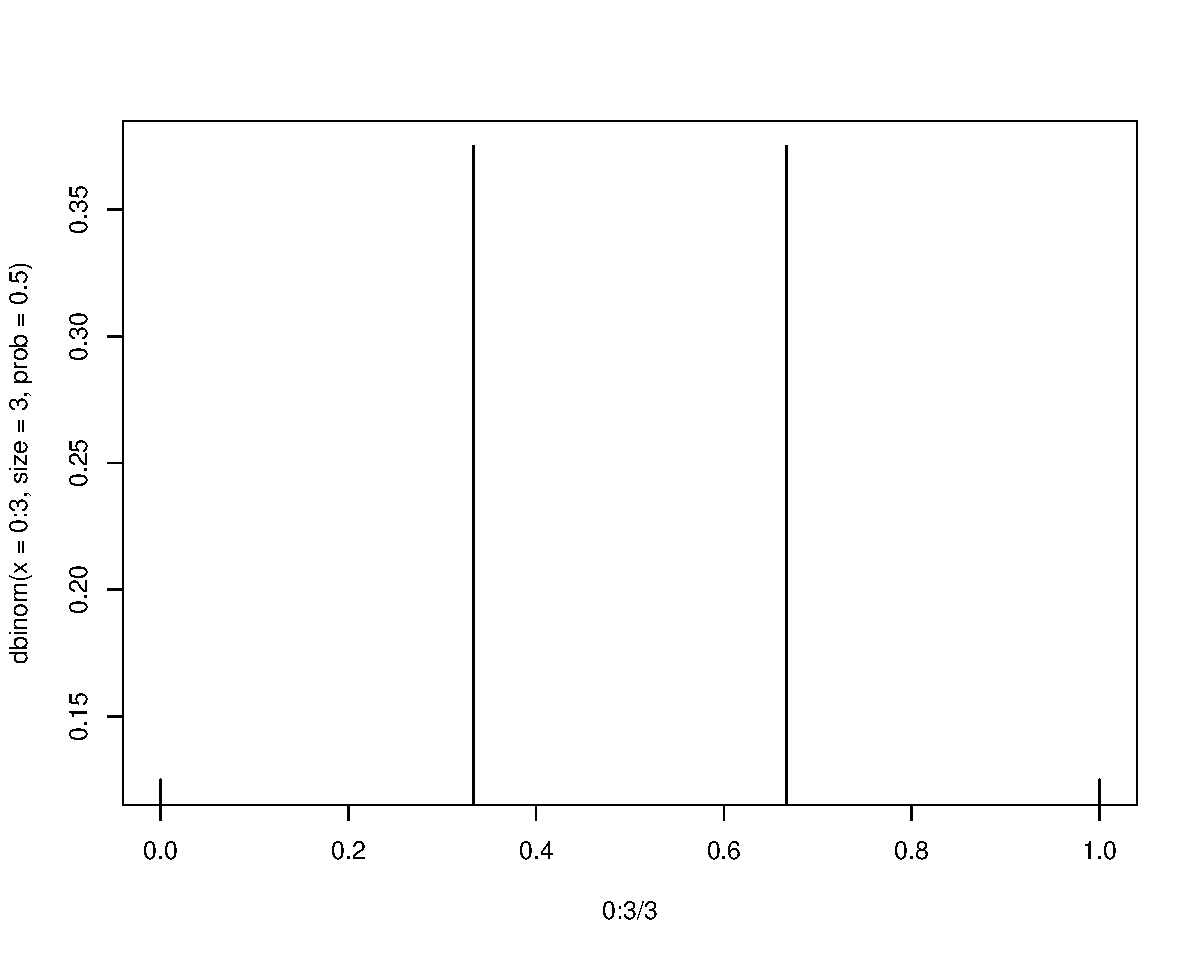
\includegraphics[width=1\linewidth]{figure/unnamed-chunk-9-1} 

}


\begin{verbatim}
## [1]  2 11
\end{verbatim}

\end{knitrout}

\end{itemize}
\end{frame}


\begin{frame}[fragile]{Confidence interval for $\mu$}
\begin{knitrout}\scriptsize
\definecolor{shadecolor}{rgb}{0.969, 0.969, 0.969}\color{fgcolor}
\begin{alltt}
\hlstd{manipulate}\hlopt{::}\hlkwd{manipulate}\hlstd{(}
\hlstd{mosaic}\hlopt{::}\hlkwd{xqpois}\hlstd{(}\hlkwd{c}\hlstd{(}\hlnum{0.025}\hlstd{,} \hlnum{0.975}\hlstd{),} \hlkwc{lambda} \hlstd{= LAMBDA),}
\hlkwc{LAMBDA} \hlstd{= manipulate}\hlopt{::}\hlkwd{slider}\hlstd{(}\hlnum{1}\hlstd{,} \hlnum{200}\hlstd{,} \hlkwc{step} \hlstd{=} \hlnum{1}\hlstd{))}
\end{alltt}

\end{knitrout}
\end{frame}



\begin{frame}[fragile]{Confidence interval for $\mu$}
\begin{itemize}
\setlength\itemsep{2em}

\item Similar to the binomial (Clopper-Pearson CI), we consider a \textit{first-principles} $100(1-\alpha)\%$ CI $[\mu_{LOWER},\: \mu_{UPPER}]$ such that  
$$P(Y \ge y \: | \: \mu_{LOWER}) = \alpha/2 \:\: \textrm{ and} \:\:  P(Y \le y \: | \: \mu_{UPPER}) = \alpha/2.$$
\item For example, the  95\% CI for $\mu$, based on $y=6,$ is  $[\underline{2.20}, \underline{13.06}].$ 
\end{itemize}
\end{frame}




\begin{frame}
\centering
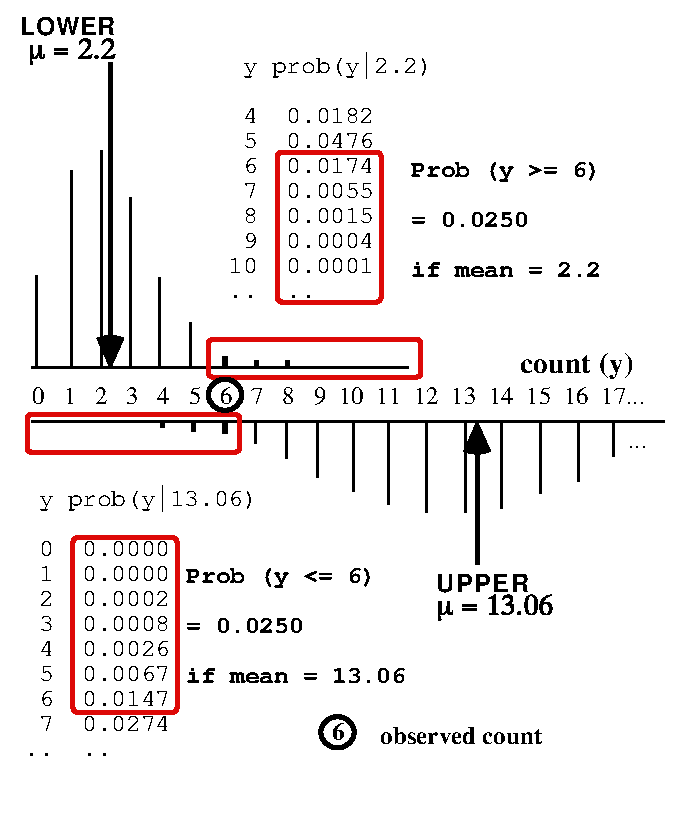
\includegraphics[width=3in,height=4in]{CI_Poisson(6).pdf}
\end{frame}


\begin{frame}[fragile]{Poisson 95\% CI for $\mu$ when $y = 6$}
\begin{knitrout}\scriptsize
\definecolor{shadecolor}{rgb}{0.969, 0.969, 0.969}\color{fgcolor}
\begin{alltt}
\hlcom{# upper limit --> lower tail needs 2.5%}
\hlstd{manipulate}\hlopt{::}\hlkwd{manipulate}\hlstd{(}
\hlstd{mosaic}\hlopt{::}\hlkwd{xppois}\hlstd{(}\hlnum{6}\hlstd{,} \hlkwc{lambda} \hlstd{= LAMBDA),}
\hlkwc{LAMBDA} \hlstd{= manipulate}\hlopt{::}\hlkwd{slider}\hlstd{(}\hlnum{0.01}\hlstd{,} \hlnum{20}\hlstd{,} \hlkwc{step} \hlstd{=} \hlnum{0.01}\hlstd{))}


\hlcom{# lower limit --> upper tail needs 2.5%}
\hlcom{# when lower.tail=FALSE, ppois doesnt include k, i.e., P(Y > k)}
\hlstd{manipulate}\hlopt{::}\hlkwd{manipulate}\hlstd{(}
\hlstd{mosaic}\hlopt{::}\hlkwd{xppois}\hlstd{(}\hlnum{5}\hlstd{,} \hlkwc{lambda} \hlstd{= LAMBDA,} \hlkwc{lower.tail} \hlstd{=} \hlnum{FALSE}\hlstd{),}
\hlkwc{LAMBDA} \hlstd{= manipulate}\hlopt{::}\hlkwd{slider}\hlstd{(}\hlnum{0.01}\hlstd{,} \hlnum{20}\hlstd{,} \hlkwc{step} \hlstd{=} \hlnum{0.01}\hlstd{))}
\end{alltt}

\end{knitrout}

\end{frame}




\begin{frame}
\frametitle{Confidence interval for $\mu$}

\begin{itemize}
\setlength\itemsep{1em}
\item For a given confidence level, there is  one CI for each value of $y$.
\item Each one can be worked out by trial and error, or -- as has been done for the last 80 years -- directly from the (exact) link between \underline{the tail areas} of the Poisson and \textbf{Gamma} distributions. 
\item These  CI's  -- for $y$ up to at least 30  -- were found in special books of statistical tables or in textbooks.
\item As you can check, $z$-based intervals are more than adequate beyond this $y$. \textbf{Today}, if you have access to \texttt{R} (or \texttt{Stata} or \texttt{SAS}) you can obtain the first principles CIs directly \textbf{for \textit{any} value of $y.$} 
\end{itemize}
\end{frame}



\begin{frame}{80\%, 90\% and 95\% CI for mean count $\mu$ if we observe \underline{0 to 30 events} in a certain amount of experience}

\tiny
\centering
\begin{tabular}{|r  | r r  |   r r  |   r r | }
$y$ & \multicolumn{2}{c}{95\%} & \multicolumn{2}{c}{90\%} & \multicolumn{2}{c}{80\%} \\
\hline
0 & 0.00 & 3.69 & 0.00 & 3.00 & 0.00 & 2.30 \\
1 & 0.03 & 5.57 & 0.05 & 4.74 & 0.11 & 3.89 \\
2 & 0.24 & 7.22 & 0.36 & 6.30 & 0.53 & 5.32 \\
3 & 0.62 & 8.77 & 0.82 & 7.75 & 1.10 & 6.68 \\
4 & 1.09 & 10.24 & 1.37 & 9.15 & 1.74 & 7.99 \\
& & & & & &  \\
5 & 1.62 & 11.67 & 1.97 & 10.51 & 2.43 & 9.27 \\
\underline{6} & \underline{2.20} & \underline{13.06} & 2.61 & 11.84 & 3.15 & 10.53 \\
7 & 2.81 & 14.42 & 3.29 & 13.15 & 3.89 & 11.77 \\
8 & 3.45 & 15.76 & 3.98 & 14.43 & 4.66 & 12.99 \\
9 & 4.12 & 17.08 & 4.70 & 15.71 & 5.43 & 14.21 \\
& & & & & &  \\
10 & 4.80 & 18.39 & 5.43 & 16.96 & 6.22 & 15.41 \\
11 & 5.49 & 19.68 & 6.17 & 18.21 & 7.02 & 16.60 \\
12 & 6.20 & 20.96 & 6.92 & 19.44 & 7.83 & 17.78 \\
13 & 6.92 & 22.23 & 7.69 & 20.67 & 8.65 & 18.96 \\
14 & 7.65 & 23.49 & 8.46 & 21.89 & 9.47 & 20.13 \\
& & & & & &  \\
15 & 8.40 & 24.74 & 9.25 & 23.10 & 10.30 & 21.29 \\
16 & 9.15 & 25.98 & 10.04 & 24.30 & 11.14 & 22.45 \\
17 & 9.90 & 27.22 & 10.83 & 25.50 & 11.98 & 23.61 \\
18 & 10.67 & 28.45 & 11.63 & 26.69 & 12.82 & 24.76 \\
19 & 11.44 & 29.67 & 12.44 & 27.88 & 13.67 & 25.90 \\
& & & & & &  \\
20 & 12.22 & 30.89 & 13.25 & 29.06 & 14.53 & 27.05 \\
21 & 13.00 & 32.10 & 14.07 & 30.24 & 15.38 & 28.18 \\
22 & 13.79 & 33.31 & 14.89 & 31.41 & 16.24 & 29.32 \\
23 & 14.58 & 34.51 & 15.72 & 32.59 & 17.11 & 30.45 \\
24 & 15.38 & 35.71 & 16.55 & 33.75 & 17.97 & 31.58 \\
\hline
\end{tabular}

\end{frame}



\begin{frame}[fragile]{95\% CI for mean count $\mu$ with \texttt{q} function}
\begin{itemize}
\setlength\itemsep{1em}
\item To obtain these in \texttt{R}	we use the  natural link between the Poisson and  the \textit{gamma} 
distributions.\footnote{
{ \tiny \href{http://www.epi.mcgill.ca/hanley/bios601/Mean-Quantile/forAccromathBackTranslate.pdf}{details found here} }} 
\item In \texttt{R}, e.g., the 95\% limits for $\mu$ based on $y=6$ are obtained as 

\begin{knitrout}\scriptsize
\definecolor{shadecolor}{rgb}{0.969, 0.969, 0.969}\color{fgcolor}
\begin{alltt}
\hlkwd{qgamma}\hlstd{(}\hlkwc{p} \hlstd{=} \hlkwd{c}\hlstd{(}\hlnum{0.025}\hlstd{,}\hlnum{0.975}\hlstd{),} \hlkwc{shape} \hlstd{=} \hlkwd{c}\hlstd{(}\hlnum{6}\hlstd{,} \hlnum{7}\hlstd{))}
\end{alltt}
\begin{verbatim}
## [1]  2.201894 13.059474
\end{verbatim}

\end{knitrout}

\item More generically, for \textit{any} $y$, as

\begin{knitrout}\scriptsize
\definecolor{shadecolor}{rgb}{0.969, 0.969, 0.969}\color{fgcolor}
\begin{alltt}
\hlkwd{qgamma}\hlstd{(}\hlkwc{p} \hlstd{=} \hlkwd{c}\hlstd{(}\hlnum{0.025}\hlstd{,}\hlnum{0.975}\hlstd{),} \hlkwc{shape} \hlstd{=} \hlkwd{c}\hlstd{(y, y}\hlopt{+}\hlnum{1}\hlstd{))}
\end{alltt}

\end{knitrout}

\end{itemize}
\end{frame}



\begin{frame}[fragile]{95\% CI for mean count $\mu$ with canned function}
\begin{itemize}
\setlength\itemsep{1em}
\item These limits can \underline{also} be found using  the canned function in \texttt{R} 

\begin{knitrout}\scriptsize
\definecolor{shadecolor}{rgb}{0.969, 0.969, 0.969}\color{fgcolor}
\begin{alltt}
\hlstd{stats}\hlopt{::}\hlkwd{poisson.test}\hlstd{(}\hlnum{6}\hlstd{)}
\end{alltt}
\begin{verbatim}
## 
## 	Exact Poisson test
## 
## data:  6 time base: 1
## number of events = 6, time base = 1, p-value = 0.0005942
## alternative hypothesis: true event rate is not equal to 1
## 95 percent confidence interval:
##   2.201894 13.059474
## sample estimates:
## event rate 
##          6
\end{verbatim}

\end{knitrout}

\end{itemize}
\end{frame}



\begin{frame}{$z$-based confidence intervals}
\scriptsize
\underline{once $\mu$ is in the upper teens}, the Poisson $\to$ the Normal

\centering
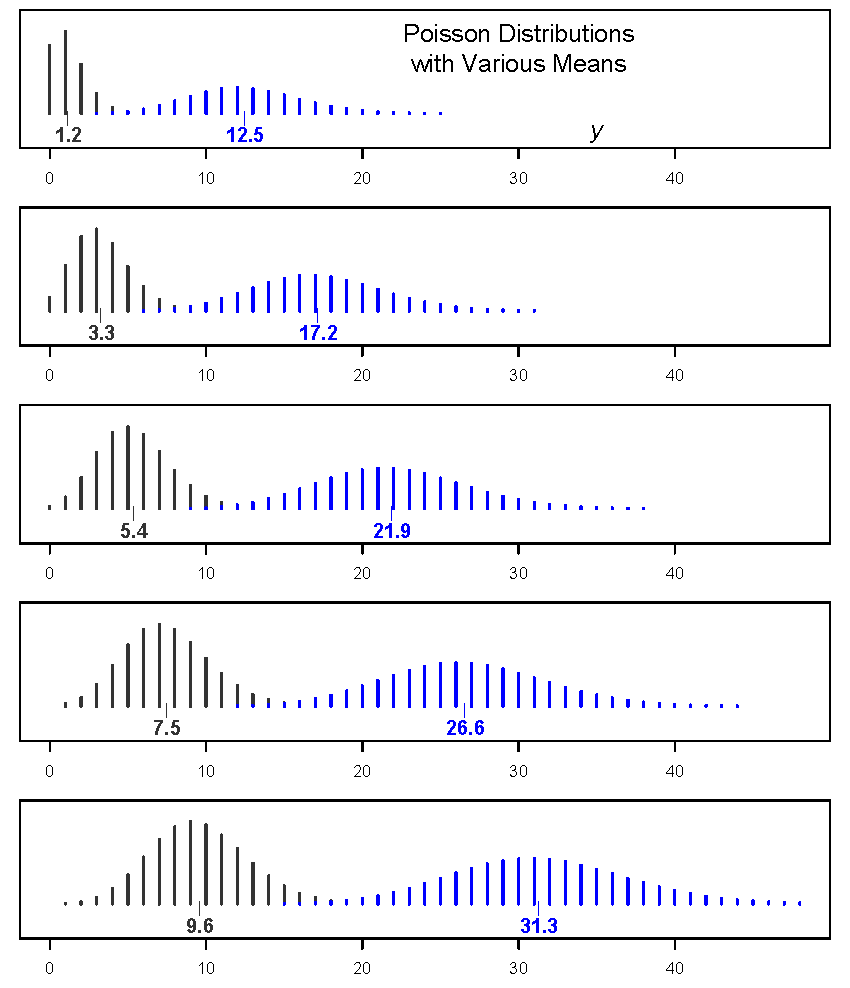
\includegraphics[scale=0.5]{Shapes.pdf}

\end{frame}


\begin{frame}{$z$-based confidence intervals}
\begin{itemize}
\setlength\itemsep{1.1em}
\item Thus, a plus/minus CI based on SE = $\hat{\sigma} =  \sqrt{\hat{\mu}} = \sqrt{y},$   is simply
$$[ \mu_{L}, \ \mu_{U}] = y  \ \pm \ z^\star \times \sqrt{y}. \ \ \ \ \ \ \ \ \ \ \ \  $$
\item Equivalently we can use the \texttt{q} function: $$qnorm(p = c(0.025, 0.975), mean = y, sd = \sqrt{y})$$
\pause 

\vspace*{-0.7cm}

\item From a single realization $y$ of a $N(\mu,\sigma_{Y})$ random variable, we can't estimate \textbf{both} $\mu$ and $\sigma_{Y}$: for a SE, we would have to use \textit{outside} information on $\sigma_{Y}$.  

\pause 

\item In the  Poisson$(\mu)$ distribution, $\sigma_{Y} = \sqrt{\mu},$ so we  calculate a ``\underline{model-based}'' SE.

%\pause 

%\item \textbf{How large a $y$?}: When $\mu  > 5,$ the distribution isn't `crowded' into the corner:   the lower tail of the Gaussian approximation doesn't  spill over the 0 boundary.
\end{itemize}

\end{frame}


\begin{frame}
\Wider[8em]{
\centering
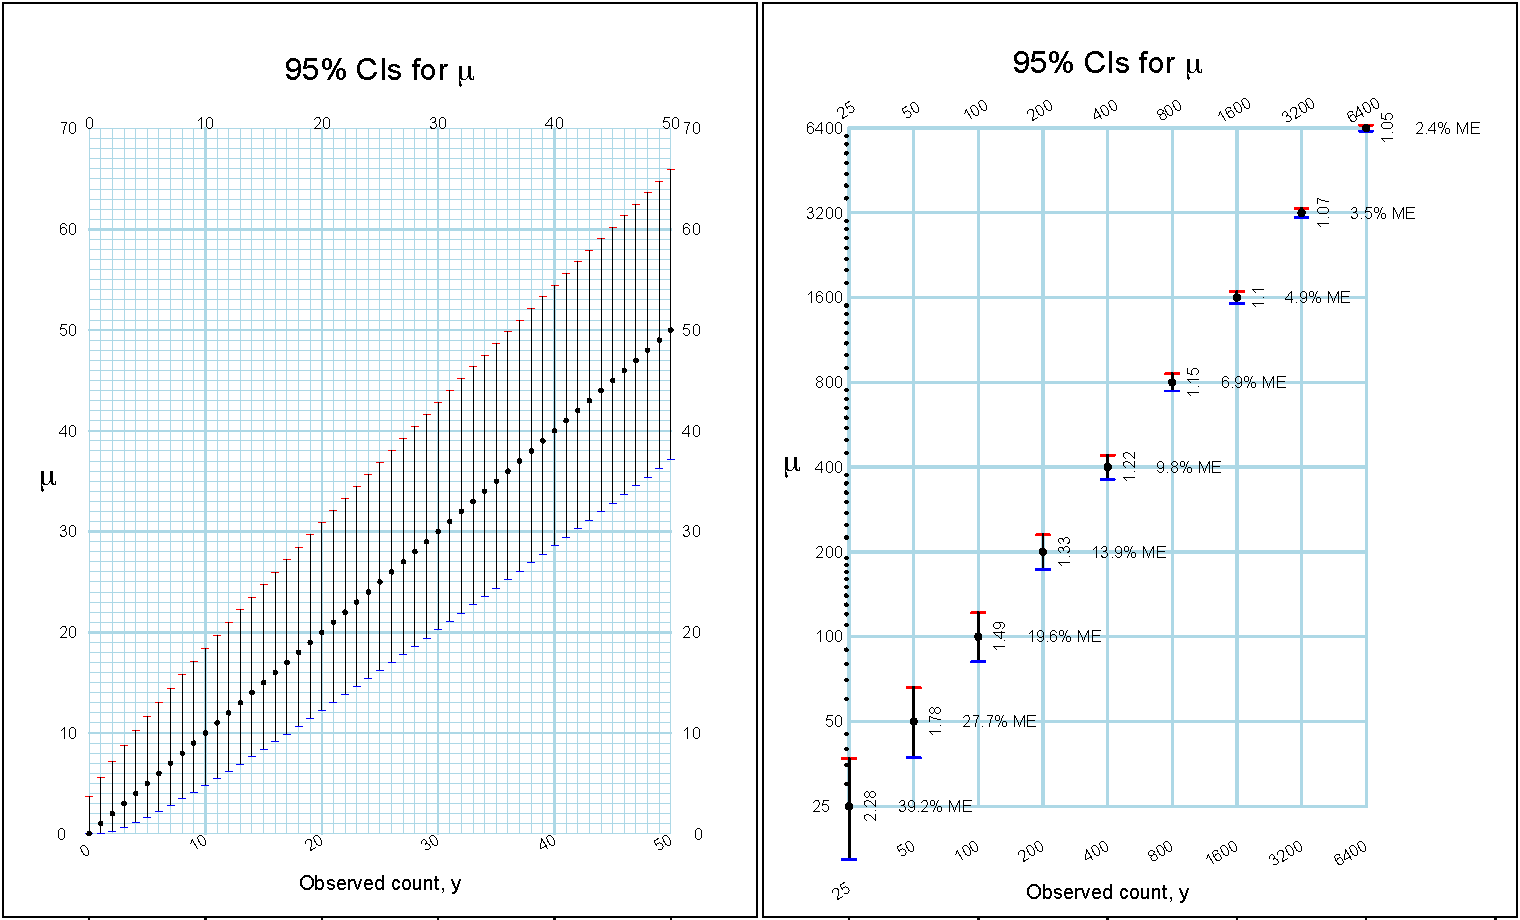
\includegraphics[width=4.9in,height=3.6in]{PoissonNomogram.pdf}
}
\end{frame}




\section{Inference regarding an event rate parameter $\lambda$, based on observed number of events $y$ in a known amount of population-time (PT)}

\begin{frame}{Rates are better for comparisons}


\begin{table}
\centering
\begin{tabular}{cc}
year & deaths ($y$) \\
\hline
1971 & 33 \\
2002 & 211 \\
\hline
\end{tabular}
\caption{Deaths from lung cancer in the age-group 55-60 in Quebec in 1971 and 2002}
\end{table} 

\pause 

\blue{A researcher asks:} Is the situation getting worse over time for lung cancer in this age group?
\pause

\vspace*{0.5in}

\red{Your reply:} \textbf{What's the denominator??}


\end{frame} 



\begin{frame}
\framedgraphic{patrick.png}
\end{frame}





\begin{frame}{Rates are better for comparisons}
\small



\begin{itemize}
\setlength\itemsep{1em}

\item So far, we have focused on inference regarding $\mu$, the expected \textbf{number} of events in the amount of experience actually studied.  

\item However, for \underline{comparison} purposes, the frequency is more often expressed as a \textbf{rate}, \textbf{intensity} or \textbf{incidence density (ID)}. \pause 
\end{itemize}

\begin{table}
\centering
\begin{tabular}{cccc}
year & deaths ($y$) & person-time (PT)  & rate ($\hat{\lambda}$)  \\
\hline
1971 & 33 & 131,200 years & 25 per 100,000 women-years\\
2002 & 211 & 232,978 years & 91 per 100,000 women-years \\
\hline
\end{tabular}
\caption{Deaths from lung cancer in the age-group 55-60 in Quebec in 1971 and 2002}
\end{table} 

\end{frame} 




\begin{frame}{Rates are better for comparisons}
\begin{itemize}
\setlength\itemsep{1.5em}

\item The \textit{statistic}, the empirical rate or empirical incidence density, is 
$$rate =\hat{ID} = \hat{\lambda} = y/\textrm{PT}.$$  

\item where $y$ is the observed number of events and PT is the amount of Population-Time in which these events were observed. 

\item We think of $\hat{ID}$ or $ \hat{\lambda}$ as a  point estimate of the (theoretical) Incidence Density \textit{parameter}, ID or $\lambda$.
\end{itemize}
\end{frame} 


\begin{frame}{CI for the rate  parameter $\lambda$}

\begin{itemize}
\item To calculate a CI for the ID parameter, we \textbf{treat the PT \underline{denominator} as a constant}, and the \textbf{\underline{numerator}, $y$,  as a Poisson random variable}, with expectation $E[y] = \mu = \lambda \times PT$, so that
\begin{align*}
\lambda &= \mu \div \textrm{PT}\\
\hat{\lambda} &= \hat{\mu} \div \textrm{PT} \\
& = y\div\textrm{ PT}
\end{align*}



\vspace*{0.3in}
\begin{equation}
\boxed{\textrm{CI for }\lambda = \{\textrm{CI for }\mu\} \div \textrm{PT}.}
\end{equation}


\end{itemize}
\end{frame}


\begin{frame}[fragile]{CI for the rate  parameter $\lambda$}


\begin{itemize}
\setlength\itemsep{1.5em}
\small
\item $y=211$ deaths from lung cancer in 2002 leads to a 95\% CI for $\mu$:

\begin{knitrout}\scriptsize
\definecolor{shadecolor}{rgb}{0.969, 0.969, 0.969}\color{fgcolor}
\begin{alltt}
\hlkwd{qgamma}\hlstd{(}\hlkwc{p} \hlstd{=} \hlkwd{c}\hlstd{(}\hlnum{0.025}\hlstd{,} \hlnum{0.975}\hlstd{),} \hlkwc{shape} \hlstd{=} \hlkwd{c}\hlstd{(}\hlnum{211}\hlstd{,} \hlnum{212}\hlstd{))}
\end{alltt}
\begin{verbatim}
## [1] 183.4885 241.4725
\end{verbatim}

\end{knitrout}

\pause 

\item From this we can calculate the 95\% CI \textbf{per 100,000 WY} for $\lambda$ using a PT=232978 years:

\begin{knitrout}\scriptsize
\definecolor{shadecolor}{rgb}{0.969, 0.969, 0.969}\color{fgcolor}
\begin{alltt}
\hlkwd{qgamma}\hlstd{(}\hlkwc{p} \hlstd{=} \hlkwd{c}\hlstd{(}\hlnum{0.025}\hlstd{,} \hlnum{0.975}\hlstd{),} \hlkwc{shape} \hlstd{=} \hlkwd{c}\hlstd{(}\hlnum{211}\hlstd{,} \hlnum{212}\hlstd{))} \hlopt{/} \hlnum{232978} \hlopt{*} \hlnum{1e5}
\end{alltt}
\begin{verbatim}
## [1]  78.75788 103.64607
\end{verbatim}

\end{knitrout}

\pause

\item $y=33$ deaths from lung cancer in 131200 women-years in 1971 leads to a 95\% CI per 100,000 WY for $\lambda$ of

\begin{knitrout}\scriptsize
\definecolor{shadecolor}{rgb}{0.969, 0.969, 0.969}\color{fgcolor}
\begin{alltt}
\hlkwd{qgamma}\hlstd{(}\hlkwd{c}\hlstd{(}\hlnum{0.025}\hlstd{,}\hlnum{0.975}\hlstd{),} \hlkwd{c}\hlstd{(}\hlnum{33}\hlstd{,}\hlnum{34}\hlstd{))} \hlopt{/} \hlnum{131200} \hlopt{*} \hlnum{1e5}
\end{alltt}
\begin{verbatim}
## [1] 17.31378 35.32338
\end{verbatim}

\end{knitrout}


\end{itemize}

\end{frame}


\begin{frame}[fragile]{CI for the rate  parameter $\lambda$ using canned function}

\begin{knitrout}\scriptsize
\definecolor{shadecolor}{rgb}{0.969, 0.969, 0.969}\color{fgcolor}
\begin{alltt}
\hlstd{stats}\hlopt{::}\hlkwd{poisson.test}\hlstd{(}\hlkwc{x} \hlstd{=} \hlnum{33}\hlstd{,} \hlkwc{T} \hlstd{=} \hlnum{131200}\hlstd{)}
\end{alltt}
\begin{verbatim}
## 
## 	Exact Poisson test
## 
## data:  33 time base: 131200
## number of events = 33, time base = 131200, p-value < 2.2e-16
## alternative hypothesis: true event rate is not equal to 1
## 95 percent confidence interval:
##  0.0001731378 0.0003532338
## sample estimates:
##   event rate 
## 0.0002515244
\end{verbatim}

\end{knitrout}

\end{frame}



\section{Test of $H_{0}: \mu = \mu_{0}$ $\quad \Leftrightarrow \quad$ $\lambda = \lambda_{0}$}


\begin{frame}{Statistical evidence and the $p$-value}

\textbf{Recall:}

\vspace*{1cm}

\begin{itemize}
\setlength\itemsep{1.2em}
\item P-Value = Prob[$y$ or more extreme $ |\:H_{0}$]

\item With `more extreme' determined by whether $H_{alt}$ is  1-sided or 2-sided. 

\item For a \textbf{formal test}, at level $\alpha$, compare this P-value with $\alpha$.
\end{itemize}

\end{frame}



\begin{frame}{Example: Cancers surrounding nuclear stations}
\small

\begin{itemize}
\setlength\itemsep{.3em}
\item Cancers in area surrounding the Douglas Point nuclear station \pause
\item Denote by $\{CY_{1},CY_{2}, \dots \}$ the numbers of Douglas Point \underline{c}hild-\underline{y}ears of experience in the various age categories that were pooled over.  
\item Denote by $\{\lambda^{Ont}_{1}, \lambda^{Ont}_{2},  \dots \}$ the age-specific leukemia incidence rates during the period studied. \pause
\item If the underlying incidence rates in Douglas Point were the same as those in the rest of Ontario, the \textbf{\textit{E}}xpected total number of cases of leukemia for Douglas Point would be

$$E = \mu_{0} = \sum_{ages} CY_{i} \times \lambda^{Ont}_{i}  = 0.57.$$
\pause
The actual total number of cases of leukemia \textbf{\textit{O}}bserved in Douglas Point was 
$$O = y = \sum_{ages} O_{i}  = 2.$$
\pause
Age \textit{Standardized Incidence Ratio (SIR)} = $O/E = 2/0.57 = 3.5.$
\end{itemize}

\end{frame}





\begin{frame}{Q: Is the $O=2$ significantly higher than $E=0.57$}

\blue{Question:}

\begin{itemize}
\setlength\itemsep{1.2em}
\item Is the $y = 2$ cases of leukemia observed in the Douglas Point experience statistically significantly \underline{higher} than the $E=0.57$  cases ``expected'' for this many child-years of  observation  if in fact the rates in Douglas Point and the rest of Ontario were the same? 
\item Or, is the $y=2$ observed in this community compatible with $H_{0}: y \sim \textrm{Poisson}(\mu = 0.57)$?
\end{itemize}

\end{frame}










\begin{frame}[fragile]{A: Is the $O=2$ significantly higher than $E=0.57$}
\small
\begin{itemize}
\setlength\itemsep{1.2em}
\item \red{Answer:} Under  $H_{0}$, the age-specific numbers of leukemias $\{y_{1}=O_{1},\: y_{2}=O_{2},\: \dots \}$ in Douglas Point can be regarded as independent Poisson random variables, so their sum $y$ can be regarded as a single Poisson random variable with $\mu=0.57$. 

\begin{knitrout}\scriptsize
\definecolor{shadecolor}{rgb}{0.969, 0.969, 0.969}\color{fgcolor}
\begin{alltt}
\hlstd{mosaic}\hlopt{::}\hlkwd{xppois}\hlstd{(}\hlnum{1}\hlstd{,} \hlkwc{lambda} \hlstd{=} \hlnum{0.57}\hlstd{,} \hlkwc{lower.tail} \hlstd{=} \hlnum{FALSE}\hlstd{)}
\end{alltt}


{\centering 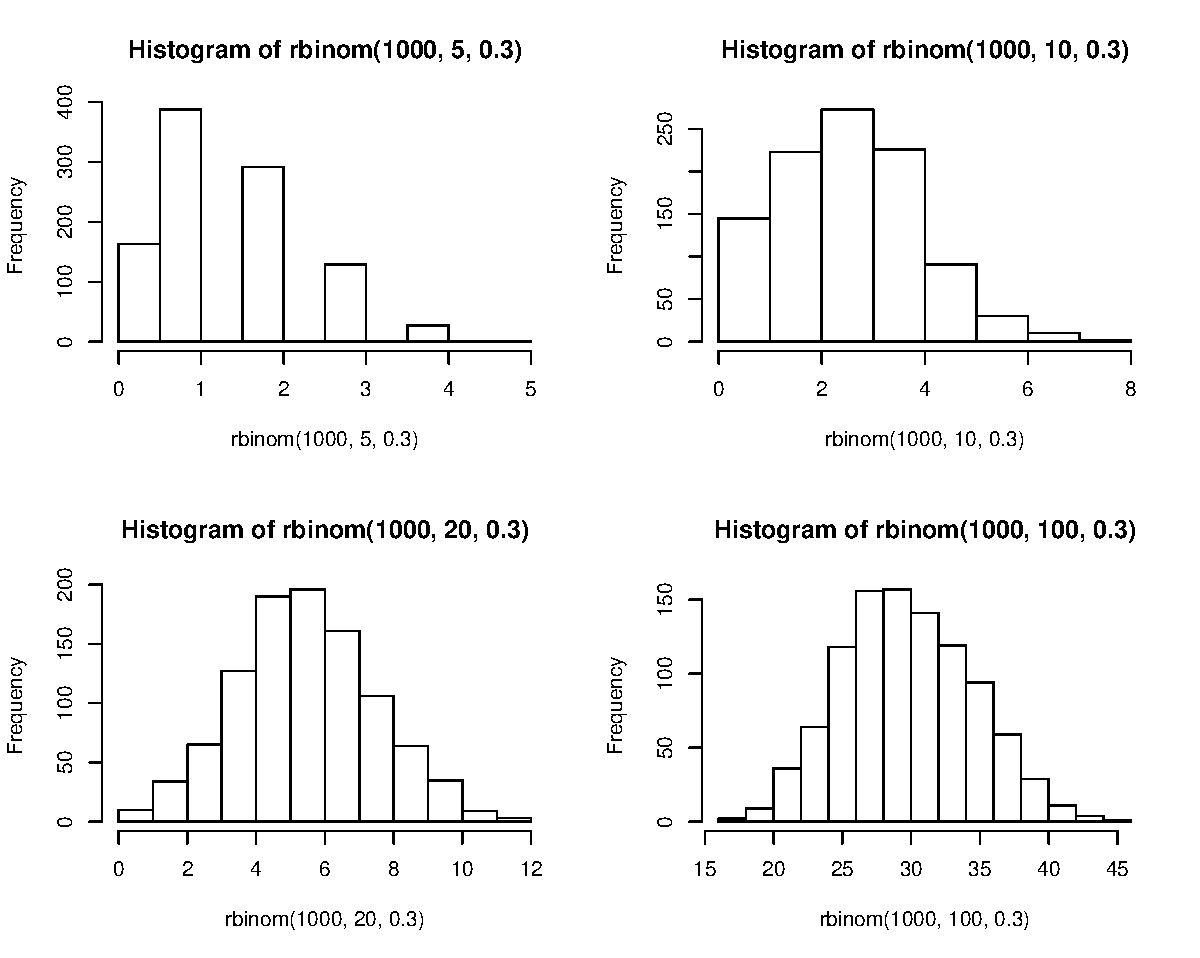
\includegraphics[width=1\linewidth]{figure/unnamed-chunk-19-1} 

}


\begin{verbatim}
## [1] 0.1121251
\end{verbatim}

\end{knitrout}


\end{itemize}

\end{frame}


\begin{frame}[fragile]{95\% CI for the SIR by hand}


\small
\begin{itemize}
\setlength\itemsep{1.2em}

\item To get the \underline{CI for the SIR}, divide the CI for Douglas Point $\mu_{DP}$ by the null $\mu_0 = 0.57$ (Ontario scaled down to the same size and age structure as Douglas Point.) We treat it as a constant because the Ontario rates used in the scaling are measured with much less sampling variability that the Douglas Point ones.

\pause 

\item The $y$ = 2 cases translates to
\begin{itemize}
\item 95\% CI for $\mu_{DP}$ $\to$ [0.24, 7.22]
\item 95\% CI for the SIR $\to$ [0.24/0.57, 7.22/0.57]=[0.4, 12.7].
\end{itemize}
\end{itemize}

\end{frame}



\begin{frame}[fragile]{95\% CI for the SIR using canned function}


\small
\begin{itemize}
\setlength\itemsep{1.2em}

\item We can \textit{trick}  \texttt{stats::poisson.test} 
to get the same CI by putting time as 0.57: 


\end{itemize}

\begin{knitrout}\scriptsize
\definecolor{shadecolor}{rgb}{0.969, 0.969, 0.969}\color{fgcolor}
\begin{alltt}
\hlstd{stats}\hlopt{::}\hlkwd{poisson.test}\hlstd{(}\hlkwc{x}\hlstd{=}\hlnum{2}\hlstd{,}\hlkwc{T}\hlstd{=}\hlnum{0.57}\hlstd{)}
\end{alltt}
\begin{verbatim}
## 
## 	Exact Poisson test
## 
## data:  2 time base: 0.57
## number of events = 2, time base = 0.57, p-value = 0.1121
## alternative hypothesis: true event rate is not equal to 1
## 95 percent confidence interval:
##   0.4249286 12.6748906
## sample estimates:
## event rate 
##   3.508772
\end{verbatim}

\end{knitrout}

\end{frame}


\section{Examples of Poisson and not-so Poisson variation}



\end{document}

{
\setbeamercolor{background canvas}{bg=}
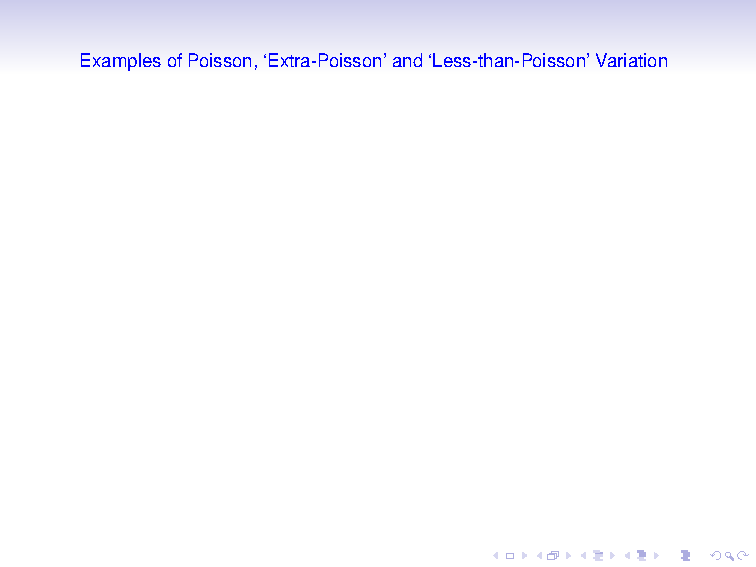
\includepdf[pages=-]{PoissonAndExtraPoissonVariation.pdf}
}


\begin{frame}{Example: Cancers surrounding nuclear stations}


\begin{itemize}
\setlength\itemsep{1.2em}
\item 
\end{itemize}

\end{frame}




\begin{frame}{Not Poisson vs. Not Poisson}


\begin{itemize}
\setlength\itemsep{1.2em}
\item  horsekicks is poisson
\item fullmoons within one day (when it comes to contrast, then compare full moon vs. other days)
\item congenital anomaly reported is
\item Daily numbers of SUdden Infant deaths is not poisson. its a seasonal thing
\end{itemize}

\end{frame}







